%Plato, Kant: aesthetics is a matter of taste
% beauty is in the eye of the beholder
\chapter{Photography \& Image Aesthetics}
\label{c2:photography_aesthetics}
\thispagestyle{empty}
\epigraph{\itshape ``Beauty is in the eye of the beholder''}
{---William Shakespeare}

%Photography offers a twofold thrill to picture-takers, There's the delight in the event that you are to capture, and there's the pleasure in reviewing the pictures days, weeks, or even years later, With a little confidence in your knowledge, skill, and experience, you'll find that arranging or discovering a photographic scene provides great satisfaction. Pictures are reminders, keys to the past—even bits of history,personal or documentary. They also express your moods, impressions, and feelings of the moment— visible statements of a very personal art. 

\section{Photography}

Photography is the practice or \textit{art} of creating images by recording the light in a light sensitive material. The official birth of photography goes back in 19th century with the invention of camera obscura(dark room), yet there is evidence within paleolithic cave artworks that this phenomenon was known  since the prehistoric age. That particular phenomena might occur from inversed projections and occurrences of camera obscura effects where light entered in a completely dark environment through tiny holes.

In ancient Greece, Aristotle first mentioned a phenomenon that he discovered during a sun eclipse. By passing sunlight through a pinhole, he could create a reversed image of the sun on the ground, as mean of observing the phenomenon without staring directly to the sun.

Much later, by the mid-17th century, with the invention of optics, camera obscura was used as tool by some artists that allowed them to paint realistic landscapes. It its very simple form, through a pinhole, a scene is projected in a dark room that the artist can draw over (Figure~\ref{c2:dark_room_photo}-a).

In 19th century, Nicephore Niepce, using a chemical compound of light-sensitive materials, created the first permanent photograph, (Figure~\ref{c2:dark_room_photo}-b) and by the start of the next century the term photography was also referred to describe a whole new industry.

\begin{figure}[h!]
    \centering  
    \subfigure[]{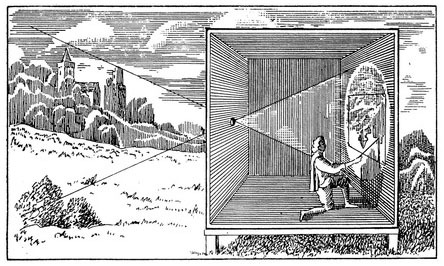
\includegraphics[width=.5\textwidth]{figures/chap2/photography/camera_obscura2}}
    \subfigure[]{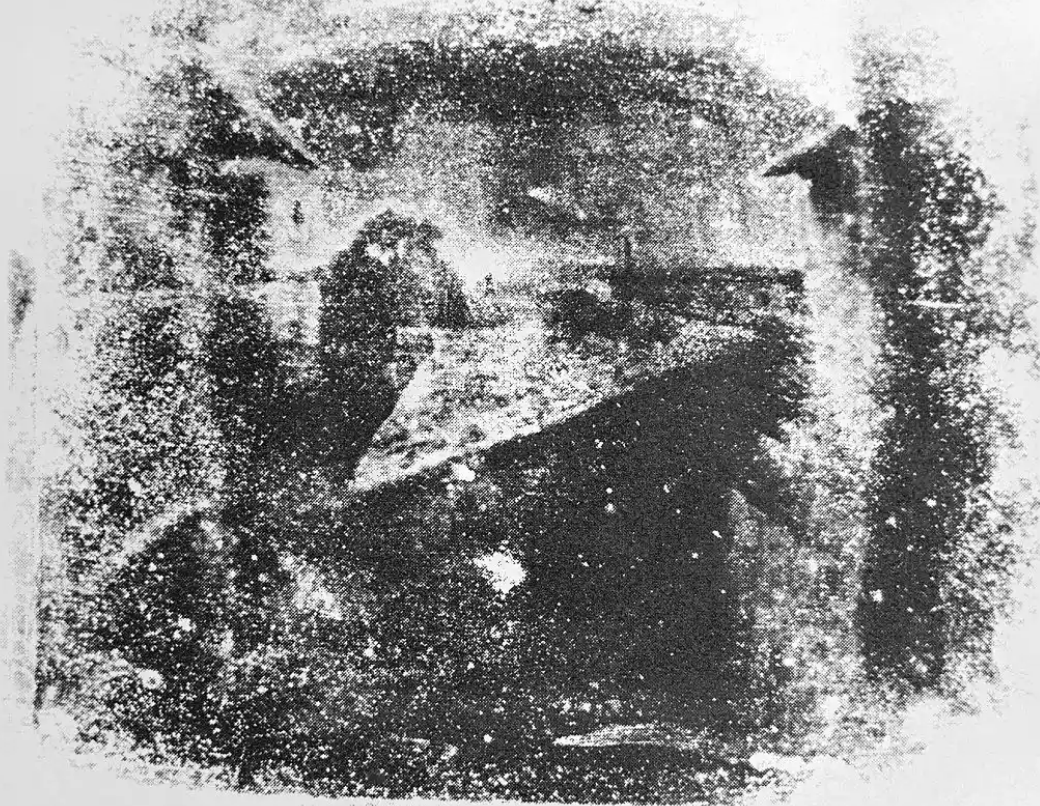
\includegraphics[width=.4\textwidth]{figures/chap2/photography/niepce}}
    \caption{(a) Camera obscura, (b) The first photograph}
    \label{c2:dark_room_photo}
\end{figure}

In the previous century, photography aside from invention became a new medium of communication, an art form and more affordable with Kodak's coloured film in 1936.

Photography as a form of art, arose from advancements in technology which enabled photographers to manipulate their image in order to form an artistic expression. Various equipment from different cameras, lenses, film and post processing techniques contributed to develop the photographer's individual genre and style of taking pictures. Since camera equipment became more modular and configurable, enabled the photographers to interact with them in order to create the picture as they wished, using techniques such as long exposures using low shutter speeds, create portraits using the different lenses or use the appropriate aperture value to put their subject in focus and make it stand-out while the background is blurred.

\subsection{Camera EXIF}

In the early film days, photographers were forced to write down the important information such aperture, shutter speed, date etc. in order to use this information in the lab during the film processsing and photo printing, a very painful process especially for new photographers.

In the era of digital photography, every modern digital camera is capable to store this information, along with all the relevant camera settings, built-in the photograph file. These settings can be utilised later in order to organise photographs, perform search and provide information about the particular camera gear and settings used.
Such metadata called EXIF(EXchangeable Image File Format) and can store a range of settings and parameters such as aperture, shutter speed, iso speed, focal length, camera model, lens type and much more.

It is much of important for a photographer who wish to find out of what ingredients a photo is made it is more than important to read this information; the latter may even be used by anyone who would like to share the information even in an image data set.

\subsection{Photography styles and camera settings}

A more experience photographer has a more firm grasp of which camera settings should be used when synthesizing a photo in order to produce the desired style. In general, there are numerous combinations to acquire the same level of illumination in a photo, but only a set of combinations to achieve a certain photography style characteristic. 
For example, in some cases an image with blurred subjects might be desired, when the synthesized frame and the camera settings are appropriately defined.
Such photography styles can be identified as long exposure shots, panning and bokeh as shown in Figure~\ref{c2:blurriness}. All of them share a similar characteristic, blurriness, but each one can only be achieved in different circumstances.

\begin{figure}[ht!]
    \centering  
    \subfigure[]{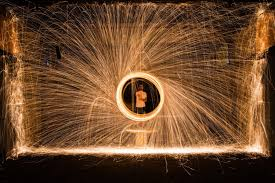
\includegraphics[width=.3\textwidth]{figures/chap2/photography/longexp}}
    \subfigure[]{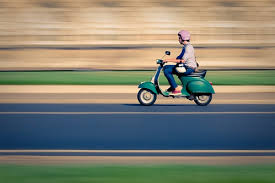
\includegraphics[width=.3\textwidth]{figures/chap2/photography/panning}}
    \subfigure[]{
\includegraphics[width=.3\textwidth]{figures/chap2/photography/bokeh}}
    \caption{Photography styles with blurry characteristics: (a) Long Exposure, (b) Panning, (c)Bokeh}
    \label{c2:blurriness}
\end{figure}

For example, producing a long exposured image, cannot be easily done handheld and under the daylight. Since a photographer wishes to smooth out a particular object in the frame, camera should be placed steady and most import use a slow shutter speed setting. A slow shutter speed will let more amount of light to enter the medium and ``burn'' the sensor or the film in the correspondent surface that the image object is reflected.

On the other hand bokeh effect, relies mostly on the aperture and lens characteristics. It requires the viewer's attention to focus on a different area, that demonstrates an artificial perspective of three dimensional world in a two dimensional image. The technical part about how camera creates shallow or large depth of field, is basically a function of lens aperture, i.e. the variable opening that allows light to enter in the medium. When reduced to its smallest size, the aperture will create an image with a large depth of field, and when widened to its largest opening it will create a shallow depth of field.
Other factor that contribute to bokeh effect are proximity to the subject and focal length.
The term \textit{bokeh} can be defined as the effect of a smooth, out-of-focus background while the main image subject stays in focus.


As the camera became a more portable medium, several movements and famous photographers emerged, such as landscape photography, documentary, photojournalism, portrait, candid and more (Figure~\ref{c2:famous}).

Photography from artistic perspective, can be seen as a superficial dimension of reality. For the majority of the people, it is a subjective interpretation of an artificially constructed and arbitrary vision.
In the next section we attempt to approach the subjectivity term from the perspective of the domain of image aesthetics.

\begin{figure}[ht!]
    \centering  
    \subfigure[]{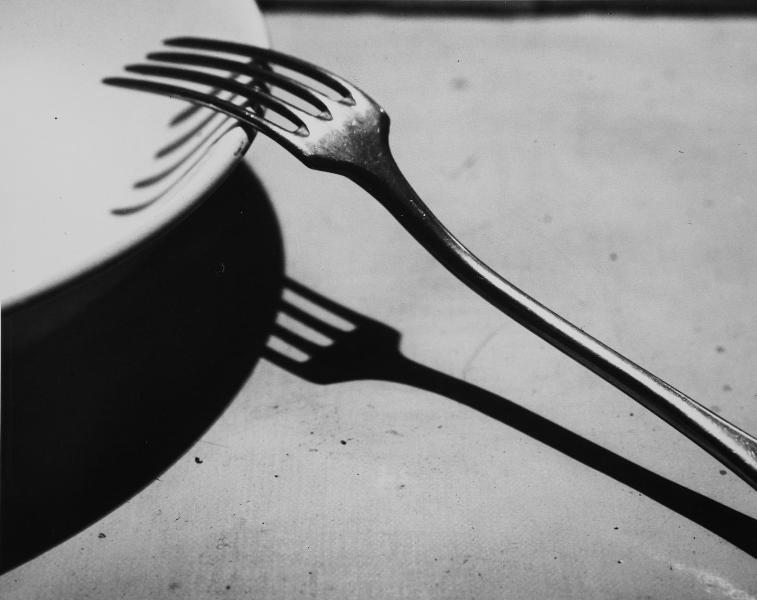
\includegraphics[width=.3\textwidth]{figures/chap2/photography/kertesz}}
    \subfigure[]{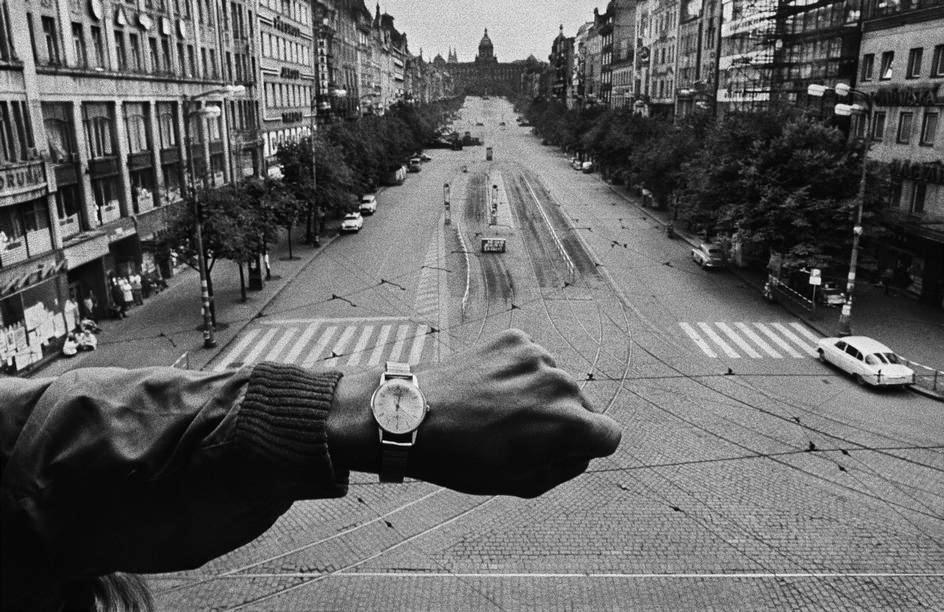
\includegraphics[width=.3\textwidth]{figures/chap2/photography/koudelka}}
    \subfigure[]{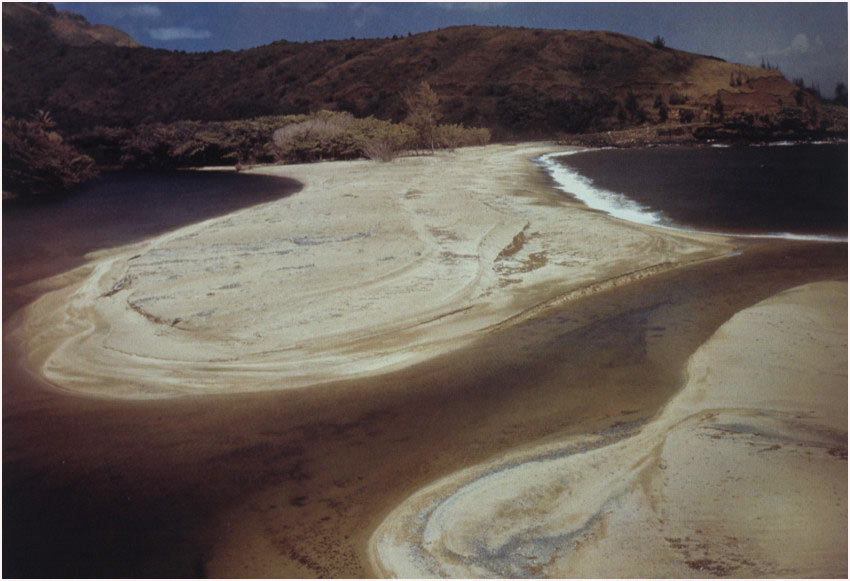
\includegraphics[width=.3\textwidth]{figures/chap2/photography/ansel_adams}}
    \caption{Famous photos with depth of field variations: (a) Andre Kertesz, (b) Josef Koudelka, (c)Ansel Adams}
    \label{c2:famous}
\end{figure}


%\chapter{Photography Style Analysis} \label{c4:intro}

\section{Aesthetics}
\label{c2:aesthetics}

The question in legitimacy of quantifying aesthetics was a subject of dispute between philosopher and art theorists and works as Jahanian's~\cite{jahanian2016quantifying} in 2016, attempted to provide a taxonomy map in order to quantify aesthetics shown in Figure~\ref{c2:aesthetics_taxonomy}.

\begin{figure}[ht!]
    \centering  
    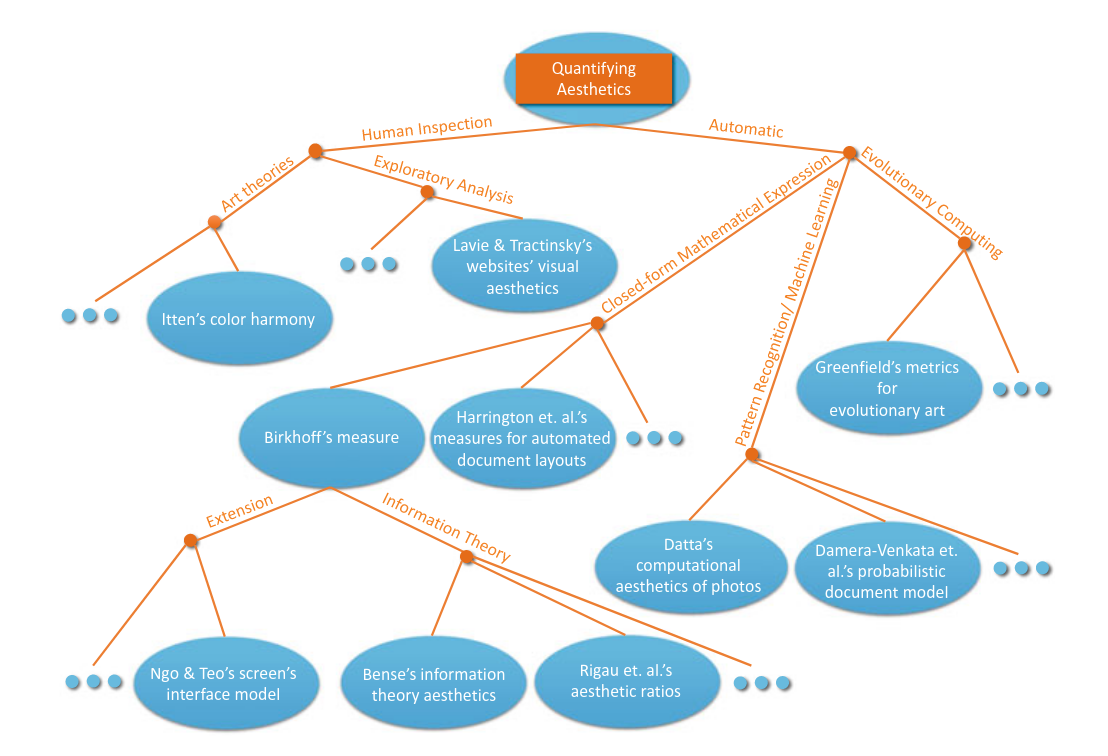
\includegraphics[width=.75\textwidth]{figures/chap2/aesthetics/taxonomy}
    \caption{Taxonomy of quantifying aesthetics}
    \label{c2:aesthetics_taxonomy}
\end{figure}

Of course, we are not the first who asked this question. In ancient years, Plato established a theory about natural and artistic beauty and the common reference that connects them, i.e., the imitation. Korsmeyer~\cite{korsmeyer1998aesthetics} summarized two opposite tenets about aesthetics. One by referring on Plato and Immanuel Kant that aesthetics is a matter of taste and the other by referring to Aristotle and Hans-Georg Gadamer, that aesthetics is a matter of cognition and learning. Yet, aesthetics is not only the study of beauty, but of taste, experience and judgement.

Based on the above taxonomy, we may find two main directions to approach it, either via human inspection or by automatic and evolutionary computations, able to measure aesthetics.


Regarding the human inspection approaches a well-known theory in visual design principles related to visual balance has been stated by a Gestalt psychologist and art theorist, Rudolf Arnheim~\cite{arnheim1960art},~\cite{marr1982vision}.
Specifically, he speculated that there exists a structural net, (Figure~\ref{c2:arnheim_net}) that contributes to a balanced spatial composition; this resembles much to the famous rule-of-thirds in photography, whereas Jahanian speculates that a good visual balance has Gaussian on the hot spots~\cite{jahanian2016deepcreativity}.

\begin{figure}[ht!]
    \centering  
    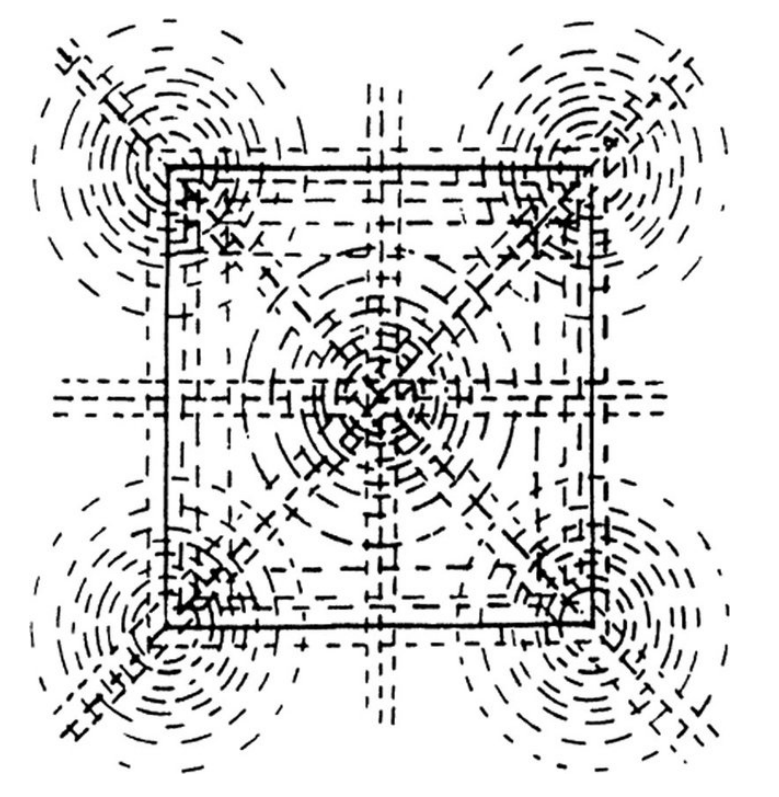
\includegraphics[width=.35\textwidth]{figures/chap2/aesthetics/arnheim_net}
    \caption{Arnheim's structural net}
    \label{c2:arnheim_net}
\end{figure}

\section{Image Aesthetics Quality Assessment(IAQA)}
\label{c2:sec_iaqa}

Image aesthetics can be defined as a subjective problem but over the latest decade image aesthetic quality assessment has demonstrated a tremendous success in variety of applications such advanced image search, retrieval and photo aesthetic enchancement.

IAQA aims to use computational techniques in order to simulate and understand human perception and cognition of the ``beauty'' and evaluate the ``beauty'' of the image.
Beauty can be described with several image aesthetic factors such content, object emphasis, light, colouring (black and white), depth of field (shallow/deep), composition (rule of thirds), motion, blur, etc.

Teaching a machine to assessing ``beauty'' is obviously a not-trivial task but recently artificial intelligence has made progress in these areas and the performance achieved in certain tasks can directly compared to humans'.
However, perceiving or creating ``beauty'' is still far away though IAQA is a crossroad for a diverse set of domains, such as computational cognition, computer vision, psychology, biology, fine arts and others~\cite{yang2019comprehensive}.

An interesting concept is the notion of \textit{aesthetic gap}~\cite{goree2021}, roughly analogous to the semantic gap in information retrieval, which separates low-level features of images like pixels and lines from high-level features like objects and symbols that humans observe in images.
Researchers have found that the feeling caused by a visual stimuli, is evoked by activations in distinct and specialized areas of the visual cortex.
Given that human perception follows a hierarchical path from the receptive field of our retina to the primal visual cortex~\cite{marr1982vision}, these activations can be categorized into the primal processing of visual stimuli inputs including colour, shapes, lines, orientation Figure~\ref{c2:vision}.

\begin{figure}[ht!]
    \centering  
    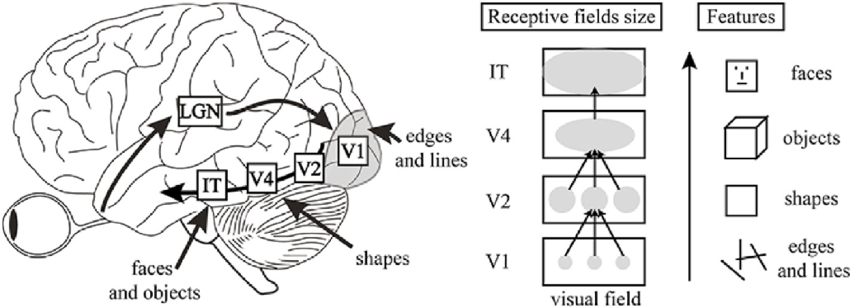
\includegraphics[width=.53\textwidth]{figures/chap2/aesthetics/human_vision}
    \caption{Perception of visual world as a hierarchical path.}
    \label{c2:vision}
\end{figure}

From the early research, IAQA does not follow the rule-based way but is treated as a data-driven learning problem. Therefore the construction of the data set is a key prerequisite to approach a certain problem.

Feature extraction techniques aim to extract high and low level features to describe and aesthetic image domain.
Traditional approaches use hand-crafted features to design specific photographic rules, image layout and objects and adopt classical machine learning algorithms to learn from those descriptions. Datta et al were determined to automatically learn from data which factors influence aesthetic value. Despite the problem ambiguity, there exist certain visual properties that make photographs more appealing than others~\cite{datta2006studying} as their concept derives from their data. They constructed a data set of 3000 images collected from \textit{photo.net} and used it to train decision trees and svms to classify images into high and low aesthetics categories based on feature variety(measures of colours, rule-of-thirds, image dimensions). However, due to the vagueness of certain photographic or art rules, hand-crafted features are often difficult to approximate them computationally.

An opposite approach for IAQA, this time from photo curation perspective proposed by Ke et al~\cite{ke2006design}, was based in computer vision rather than psychological aesthetics, by measuring image noise and degradation. Their method utilizes images and ratings from the photo challenge of \textit{DPChallenge.com}, which are used to extract features such edge and colour histograms and Fourier transformation based blur metrics in order to train a Naive Bayes classifier.

Later, a variety of other techniques emerged, proposing different image features like GIST or SIFT descriptors from Marchesotti et al.~\cite{marchesotti2011assessing} which argued on the non-exhaustive nature of hand-crafted features. The latter are heuristically generated and have shown generalization limitations in several problems and domains of application.


Based on a recent survey on computational aesthetic evaluation in visual art images~\cite{zhang2021comprehensive}, two research methods have been set, so far.
The first is based on conventional approaches such as the aforementioned ones, i.e., by using handcrafted features, while within the second 
aesthetic judgement is carried through deep learning techniques (Figure~\ref{c2:aesthetics_methods}). We shall provide further details regarding the latter in Section~\ref{c3:section_aesthetics_deep}.


\begin{figure}[h!]
    \centering  
    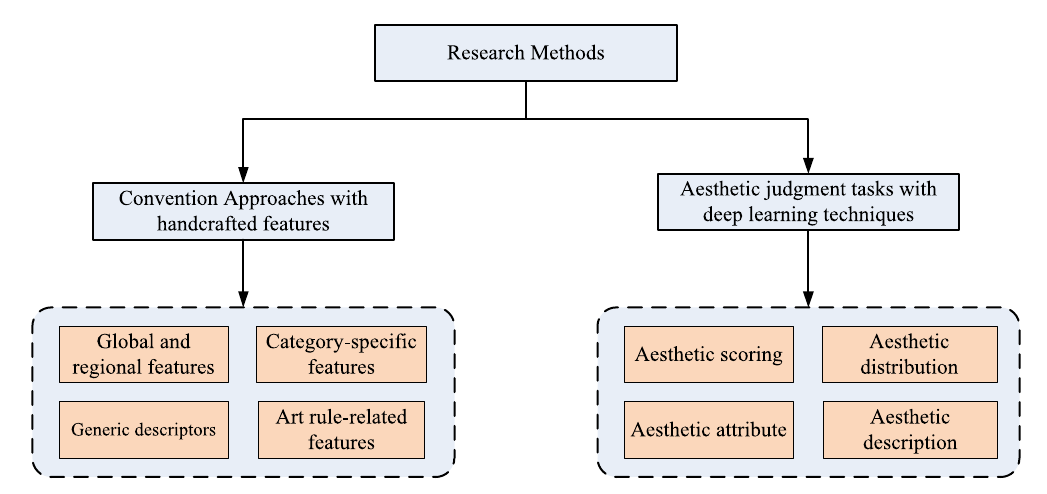
\includegraphics[width=.6\textwidth]{figures/chap2/aesthetics/methods}
    \caption{Research methods in aesthetic evaluation classification.}
    \label{c2:aesthetics_methods}
\end{figure}

So far we have covered the origins and latest developments in photography, analyzing popular photography styles and how they are related to general camera technical aspects. In addition, we have presented the philosophical and psychological background in aesthetics and traced the evolution of IAQA.
